\documentclass[11pt]{article}
\usepackage[margin=1.1in]{geometry}
\usepackage{amsmath,amssymb}
\usepackage{booktabs}
\usepackage{tikz}
\usetikzlibrary{arrows.meta,positioning}
\usepackage[hidelinks]{hyperref}

\title{Attention, Briefly}
\author{An example paper for \texttt{tex}}
\date{}

\begin{document}
\maketitle

\begin{abstract}
Self-attention lets every token in a sequence read from every other token. This note derives the operation from one question, works through its cost, and shows why long contexts are expensive. It exists to show what a paper looks like in \texttt{tex}: edit any line on the left and the PDF on the right updates a moment later.
\end{abstract}

\section{The question attention answers}\label{sec:question}

A model reading the sentence ``the cat sat because it was tired'' has to decide what \emph{it} refers to. Attention answers that question with arithmetic: each token builds a \emph{query}, every token offers a \emph{key} and a \emph{value}, and a token's output is the average of all values weighted by how well its query matches each key \cite{vaswani2017}.

\begin{figure}[ht]
\centering
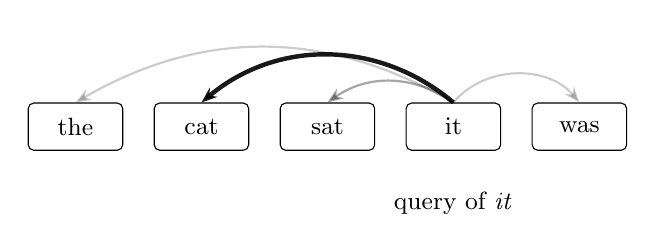
\begin{tikzpicture}[
  tok/.style={draw, rounded corners=2pt, minimum width=12mm, minimum height=6mm, font=\small},
  arr/.style={-{Stealth[length=2mm]}, thick}]
  \foreach \w/\x in {the/0, cat/1.6, sat/3.2, it/4.8, was/6.4}
    \node[tok] (\w) at (\x,0) {\w};
  \draw[arr, opacity=0.9, line width=1.6pt] (it.north) to[bend right=40] (cat.north);
  \draw[arr, opacity=0.35] (it.north) to[bend right=35] (sat.north);
  \draw[arr, opacity=0.2] (it.north) to[bend right=30] (the.north);
  \draw[arr, opacity=0.2] (it.north) to[bend left=50] (was.north);
  \node[font=\small, below=4mm of it] {query of \emph{it}};
\end{tikzpicture}
\caption{The token \emph{it} attends to every token; line weight is the attention weight.
Most of the weight lands on \emph{cat}.}
\label{fig:weights}
\end{figure}

\section{The operation}\label{sec:op}

Stack the queries, keys and values of $n$ tokens into matrices $Q, K, V \in \mathbb{R}^{n \times d}$. Then
\begin{equation}\label{eq:attn}
  \operatorname{Attention}(Q,K,V) = \operatorname{softmax}\!\left(\frac{QK^{\top}}{\sqrt{d}}\right) V .
\end{equation}
The product $QK^{\top}$ scores every pair of tokens, the softmax turns each row of scores into weights that sum to one, and multiplying by $V$ mixes the values. Dividing by $\sqrt{d}$ keeps the scores from growing with the width $d$, which would push the softmax into a near one-hot choice (Figure~\ref{fig:weights} shows a soft one).

\section{What it costs}\label{sec:cost}

Equation~\eqref{eq:attn} builds an $n \times n$ score matrix, so both work and memory grow with the square of the sequence length. Table~\ref{tab:cost} puts numbers on it for a single head with $d = 128$ and 16-bit scores.

\begin{table}[ht]
\centering
\begin{tabular}{rrr}
\toprule
Tokens $n$ & Score entries $n^2$ & Score memory \\
\midrule
1\,024   & $1.0 \times 10^{6}$ & 2\,MB \\
8\,192   & $6.7 \times 10^{7}$ & 134\,MB \\
131\,072 & $1.7 \times 10^{10}$ & 34\,GB \\
\bottomrule
\end{tabular}
\caption{Doubling the context quadruples the score matrix.}
\label{tab:cost}
\end{table}

Sparse patterns \cite{child2019} and kernels that never materialise the full matrix are the two standard ways out; Section~\ref{sec:question} explains why the model wants the long context in the first place.

\begin{thebibliography}{9}
\bibitem{vaswani2017} A.~Vaswani et al. Attention is all you need. \emph{NeurIPS}, 2017.
\bibitem{child2019} R.~Child et al. Generating long sequences with sparse transformers.
  \emph{arXiv:1904.10509}, 2019.
\end{thebibliography}

\end{document}
